%
% teil2.tex -- Beispiel-File für teil2 
%
% (c) 2020 Prof Dr Andreas Müller, Hochschule Rapperswil
%
\section{FM und Besselfunktion 
\label{fm:section:proof}}
\rhead{Herleitung}
Die momentane Trägerkreisfrequenz \(\omega_i\) wie schon in (ref) beschrieben ist, bringt die Vorigen Kapittel beschreiben. (Ableitung \(\frac{d \varphi(t)}{dt}\) mit sich).
Diese wiederum kann durch \(\beta\sin(\omega_mt)\) ausgedrückt werden, wobei es das Modulierende Signal \(m(t)\) ist.
Somit haben wir unser \(x_c\) welches 
\[
\cos(\omega_c t+\beta\sin(\omega_mt))
\]
ist.
\subsection{Herleitung}
Das Ziel ist es Unser moduliertes Signal mit der Besselfunktion so auszudrücken:
\begin{align}
    \cos(\omega_ct+\beta\sin(\omega_mt))
    &=
    \sum_{k= -\infty}^\infty J_{k}(\beta) \cos((\omega_c+k\omega_m)t)
    \label{fm:eq:proof}
\end{align}
Doch dazu brauchen wir die Hilfe der Additionsthoerme 
\begin{align}
    \cos(A + B) 
    &= 
    \cos(A)\cos(B)-\sin(A)\sin(B)
    \label{fm:eq:addth1}
    \\
    2\cos (A)\cos (B)
    &=
    \cos(A-B)+\cos(A+B)
    \label{fm:eq:addth2}
    \\
    2\sin(A)\sin(B)
    &=
    \cos(A-B)-\cos(A+B)
    \label{fm:eq:addth3}
\end{align}
und die drei Besselfunktions indentitäten,
\begin{align}
    \cos(\beta\sin\phi)
    &=
    J_0(\beta) + 2\sum_{k=1}^\infty J_{2k}(\beta) \cos(2k\phi)
    \label{fm:eq:besselid1}
    \\
    \sin(\beta\sin\phi)
    &=
    J_0(\beta) + 2\sum_{k=1}^\infty J_{2k+1}(\beta) \cos((2k+1)\phi)
    \label{fm:eq:besselid2}
    \\
    J_{-n}(\beta) &= (-1)^n J_n(\beta)
    \label{fm:eq:besselid3}
\end{align}
welche man im Kapitel (ref), ref, ref findet.
\newline
Mit dem \refname{fm:eq:addth1} wird aus dem modulierten Signal
\[
\cos(\omega_c t + \beta\sin(\omega_mt))
\]
das Signal
\[
    \cos(\omega_c t)\cos(\beta\sin(\omega_m t))-\sin(\omega_c)\sin(\beta\sin(\omega_m t)).
    \label{fm:eq:start}
\]
Zu beginn wird der erste Teil 
\[
    \cos(\omega_c)\cos(\beta\sin(\omega_mt))  
\]
mit hilfe der Bessel indentität \ref{fm:eq:besselid1} zum
\[
    J_0(\beta)\cos(\omega_c) + \sum_{k=1}^\infty J_{2k}(\beta) 2\cos(\omega_c t)\cos(2k\omega_m t)
\]
\newline
TODO 2 und \(\cos( )\) in lime.
wobei mit dem \colorbox{lime}{Additionstheorem} \ref{fm:eq:addth2} zum
\[
    J_0(\beta)\dot \cos(\omega_c t) + \sum_{k=1}^\infty J_{2k}(\beta) \{ \cos((\omega_c - 2k\omega_m) t)+\cos((\omega_c + 2k\omega_m) t) \}
\]
wird.
Wenn dabei \(2k\) durch alle geraden Zahlen von \(-\infty \to \infty\) mit \(n\) substituiert erhält man den vereinfachten Term
\[
    \sum_{n\, gerade} J_{n}(\beta) \cos((\omega_c + n\omega_m) t)
    \label{fm:eq:gerade}
\]
\newline
nun zum zweiten Teil des Term \ref{fm:eq:start} 
\[
    \sin(\omega_c)\sin(\beta\sin(\omega_m t)).
\]
Dieser wird mit der \ref{fm:eq:besselid2} Bessel indentität zu
\[
    J_0(\beta) \dot \sin(\omega_c t) + \sum_{k=1}^\infty J_{2k+1}(\beta) 2\sin(\omega_c t)\cos((2k+1)\omega_m t).
\]
Auch hier wird ein Additionstheorem \ref{fm:eq:addth3} gebraucht um aus dem Sumanden diesen Term 
\[
    J_0(\beta) \dot \sin(\omega_c) + \sum_{k=1}^\infty J_{2k+1}(\beta) \{ \underbrace{\cos((\omega_c-(2k+1)\omega_m) t)}_{Teil1} - \cos((\omega_c+(2k+1)\omega_m) t) \}
\]zu gewinnen.
Wenn dabei \(2k +1\) durch alle ungeraden Zahlen von \(-\infty \to \infty\) mit \(n\) substituiert.
Zusätzlich dabei noch die letzte Bessel indentität \ref{fm:eq:besselid3} brauchen, ist bei allen ungeraden negativen \(n : J_{-n}(\beta) = -1 J_n(\beta)\).
Somit wird Teil1 zum negativen Term und die Summe vereinfacht sich zu
\[
     \sum_{n\, ungerade} -1 J_{n}(\beta) \cos((\omega_c + n\omega_m) t).
     \label{fm:eq:ungerade}
\]
Substituiert man nun noch \(n \text{mit} -n \) so fällt das \(-1\) weg.
Beide Teile \ref{fm:eq:gerade} Gerade und \ref{fm:eq:ungerade} Ungerade ergeben zusammen
\[
    \cos(\omega_ct+\beta\sin(\omega_mt))
    =
    \sum_{k= -\infty}^\infty J_{k}(\beta) \cos((\omega_c+k\omega_m)t).
\]
Somit ist \ref{fm:eq:proof} bewiesen.
\newpage
\subsection{Bessel und Frequenzspektrum}
Um sich das ganze noch einwenig Bildlicher vorzustellenhier einmal die Besselfunktion \(J_{k}(\beta)\) in geplottet.
\begin{figure}
	\centering
%	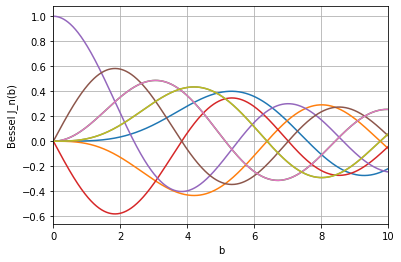
\includegraphics[width=0.5\textwidth]{/home/joshua/Documents/SeminarSpezielleFunktionen/buch/papers/fm/FM presentation/images/bessel.png}
	\caption{Bessle Funktion \(J_{k}(\beta)\)}
	\label{fig:bessel}
\end{figure}
TODO Grafik einfügen,
\newline
Nun einmal das Modulierte FM signal im Frequenzspektrum mit den einzelen Summen dargestellt

TODO
Hier wird beschrieben wie die Bessel Funktion der FM im Frequenzspektrum hilft, wieso diese gebrauch wird und ihre Vorteile.
\begin{itemize}
    \item Zuerest einmal die Herleitung von FM zu der Besselfunktion
    \item Im Frequenzspektrum darstellen mit Farben, ersichtlich machen. 
    \item Parameter tuing der Trägerfrequenz, Modulierende frequenz und Beta. 
\end{itemize}


%\subsection{De finibus bonorum et malorum
%\label{fm:subsection:bonorum}}



